\documentclass[12pt,a4paper]{article}
\usepackage[brazil]{babel}
\usepackage[utf8]{inputenc}
\usepackage[T1]{fontenc}
\usepackage{graphicx} % para inserção de figuras


\author{Universidade Católica Don Bosco \\ Computação Gráfica - Engenharia da Computação \\Uéliton Freitas}
\title{Lista de Exercícios I}
\begin{document}
\maketitle


\begin{enumerate}
	\item Na Figura \ref{Fig:are} é apresentado o relacionamento entre as áreas relacionadas. Descreva em quais relacionamentos as seguintes áreas atuam, como elas interagem e dê pelo menos dois exemplos práticos de cada uma:
	\begin{itemize}
		\item Comutação Gráfica.
		\item Processamento de Imagens.
		\item Visão Computacional.
	\end{itemize}
	
		\begin{figure}[!h]
		\label{Fig:are}
			\begin{center}
			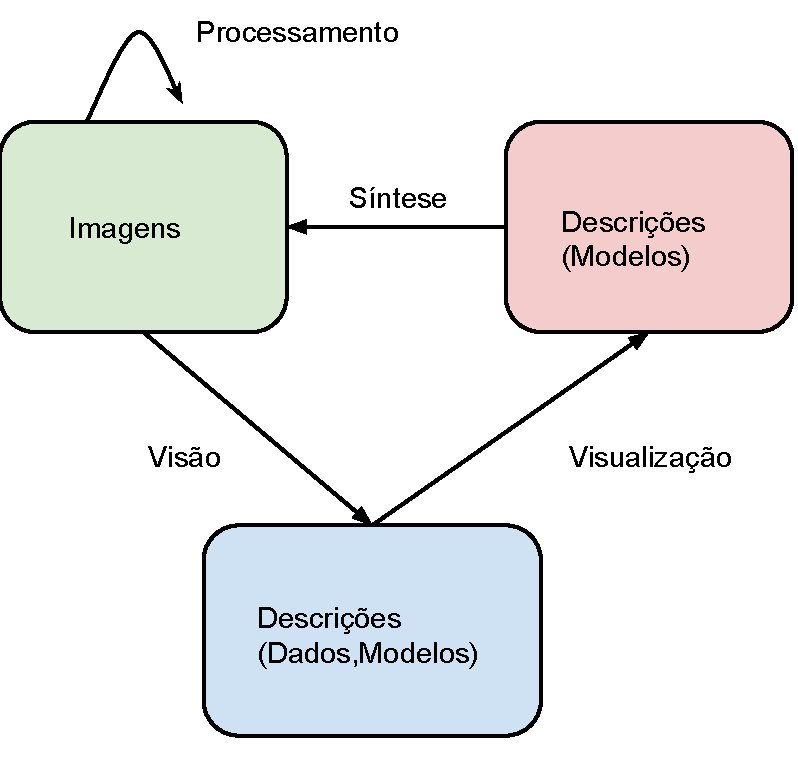
\includegraphics[width=0.48\textwidth]{Are}
			\caption{Relacionamento entre as áreas.}
			
			\end{center}
	\end{figure}
	

	\item Quais sãs vantagens e desvantagens de dispositivos vetoriais?	
	
	\item O que  é vertical e horizontal retrace?

	\item O que  é um frame buffer? Para que serve a profundidade do f.b?

	\item O que  é uma Look-up table? Qual  é a sua utilidade? Dê um exemplo de uso.

	\item Quais são as vantagens e desvantagens de dispositivos matriciais?

	\item Considere um triângulo composto pelos pontos $(0,0)$, $(1,0)$ e $(0.5,1)$. Apresente a matriz de transformação que rotacione o triângulo em 90 graus (sentido anti horário) utilizando como pivô de rotação o ponto (0.5,0.5). Calcule novos pontos do triângulo após essas transformações.

	\item Considere o mesmo triângulo composto pelos pontos $(0,0)$, $(1,0)$ e $(0.5,1)$
e apresente a matriz de transformação e as coordenadas do triângulo ao rotacioná-lo em 30 graus (sentido anti-horário) utilizando como pivô de rotação o ponto $(0.5, 0.5)$ e transladando em $T(1,1)$.	

	\item Apresente a matriz de transformação para um novo sistema de coordenadas $y’$ e $x’$ onde o ponto de origem está em (1,1) e a rotação  é de 45 graus (sentido anti horário).
	
	\item Calcule as coordenadas do triângulo composto pelos pontos (0,0), (1,0) e
(0.5,1) no sistema de coordenadas do exercício anterior.

	\item Apresente o pipeline de visualização 2D e explique cada uma de suas 4
etapas e o que representam os 5 sistemas de coordenadas.

	\item Calcule a matriz de transformação de um sistema de coordenadas do
mundo para um sistema de coordenadas normalizadas da view port.

	\item Considere um segmento de reta composto pelos pontos (0,-1) e (2,2). Faça
os recortes necessários para uma janela de recorte com $(x_{min} = 0, y_{min} =0)$ e $(x_{max} = 1, y_{max} = 1)$ utilizando o algoritmo de Cohen-Sutherland.

	\item Considere a seguinte ordem de recortadores utilizando o algoritmo de Sutherland-Hodgman: Esquerda, Direita, Baixo e Cima. Apresente as saídas de cada recortador ao processar um polígono convexo composto pelos seguintes pontos: (0.5,-0.5), (1,0.5), (0.5, 1.5), (-0.5,0.5).
	
	\item Considere um Cubo em um espaço 3D posicionado em (0,0,0) com o vetor de view up igual a (0,1,0). Calcule todos os passos para rotacionar este cubo em 60 graus utilizando o eixo de rotação que contém os pontos (1,1,1) e (2,2,2).
	
	\item Apresente a matriz de transformação para a mudança de coordenada em um sistema 3D composto com origem em (2,2,2) e com os vetores (1,1,3),(-1,1,0) e (-3,-3,2).

\end{enumerate}


\end{document}